\documentclass[11pt,a4paper,oneside]{article}
\usepackage{preamble}
\title{Poset of Mesh Patterns}

\begin{document}
	\maketitle

%\section{Introduction}

\section{The Poset of Mesh Patterns}

Mesh patterns were first introduced in \cite{Bra11} and a concept mesh pattern containment was introduced in \cite{TU17}. A mesh pattern is of the form $p=(\cl(p),\sh(p))$, where $\cl(p)$ is a permutation and $\sh(p)$ is a set of coordinates corresponding to the boxes that are shaded, where $(i,j)$ denotes the box $[i,i+1]\times[j,j+1]$, see \cref{fig:132}. We also denote $p$ by $\cl(p)^{\sh(p)}$, for example $132^\emptyset$ is the mesh pattern on $132$ with no shaded boxes. Let $G(p)$ be the set of coordinates of the points of $p$.

We let $|\cl(p)|$ represent the length of $\cl(p)$ and $|\sh(p)|$ the size of $\sh(p)$, and define the length of $p$ as $|\cl(p)|$. We define the \emph{rank} of $p$ as $|\pi|+|P|$, that is, the number of points plus the number of shaded boxes.


\begin{figure}\centering\begin{tikzpicture}
\patt{1}{3}{1,3,2}[0/1,0/0,2/2][][][][][4]
\node (inv) at (0,-2){};
\end{tikzpicture}
\caption{The Mesh pattern $(132,\{(0,0),(0,1),(2,2)\})$, or equivalently $132^{(0,0),(0,1),(2,2)}$.}\label{fig:132}\end{figure}

Given two classical permutations $\sigma$ and $\pi$, an occurrence of $\sigma$ in $\pi$ is a map $\alpha:[|\sigma|]\rightarrow[|\pi|]$ such that $\alpha(1)\alpha(2)\ldots\alpha(|\sigma|)$ has the same relative order of size as $\sigma$. Given any letter $b=\sigma_i$ let $\hat{\alpha}(b)=\pi_{\alpha(i)}$, so $\hat{\alpha}$ maps the value of a letter in $\sigma$ to its value in $\pi$ under the map $\alpha$.

Using the notion of pattern occurrence we can define a partial order on permutations where $\sigma\leP\pi$ if there is an occurrence of $\sigma$ in $\pi$. Let $\mathcal{P}$ be the poset of all permutations with the partial order $\leP$, we call this the \emph{classical permutation poset}.

We can extend this definition to define an occurrence in a mesh pattern. Consider a pair of mesh patterns $m$ and $p$ and an occurrence $\alpha$ of $\cl(m)$ in $\cl(p)$. Define $R^\alpha_{i,j}=[\alpha(i),\alpha(i+1)]\times[\hat{\alpha}(j),\hat{\alpha}(j+1)]$, this is the area in $p$ that corresponds to the box $(i,j)$ in $m$ according to $\alpha$

An \emph{occurrence} of $m$ in $p$ is an occurrence $\alpha$ of $\cl(m)$ in $\cl(p)$ satisfying $\bigcup_{(i,j)\in \sh(m)}R^\alpha_{i,j}\subseteq\sh(p)$ and $G(p)\cap\bigcup_{(i,j)\in \sh(m)}R^\alpha_{i,j}=\emptyset$. This is equivalent to saying every shaded point in $m$ corresponds to a fully shaded area in $p$ that contains no points.

\begin{figure}\centering
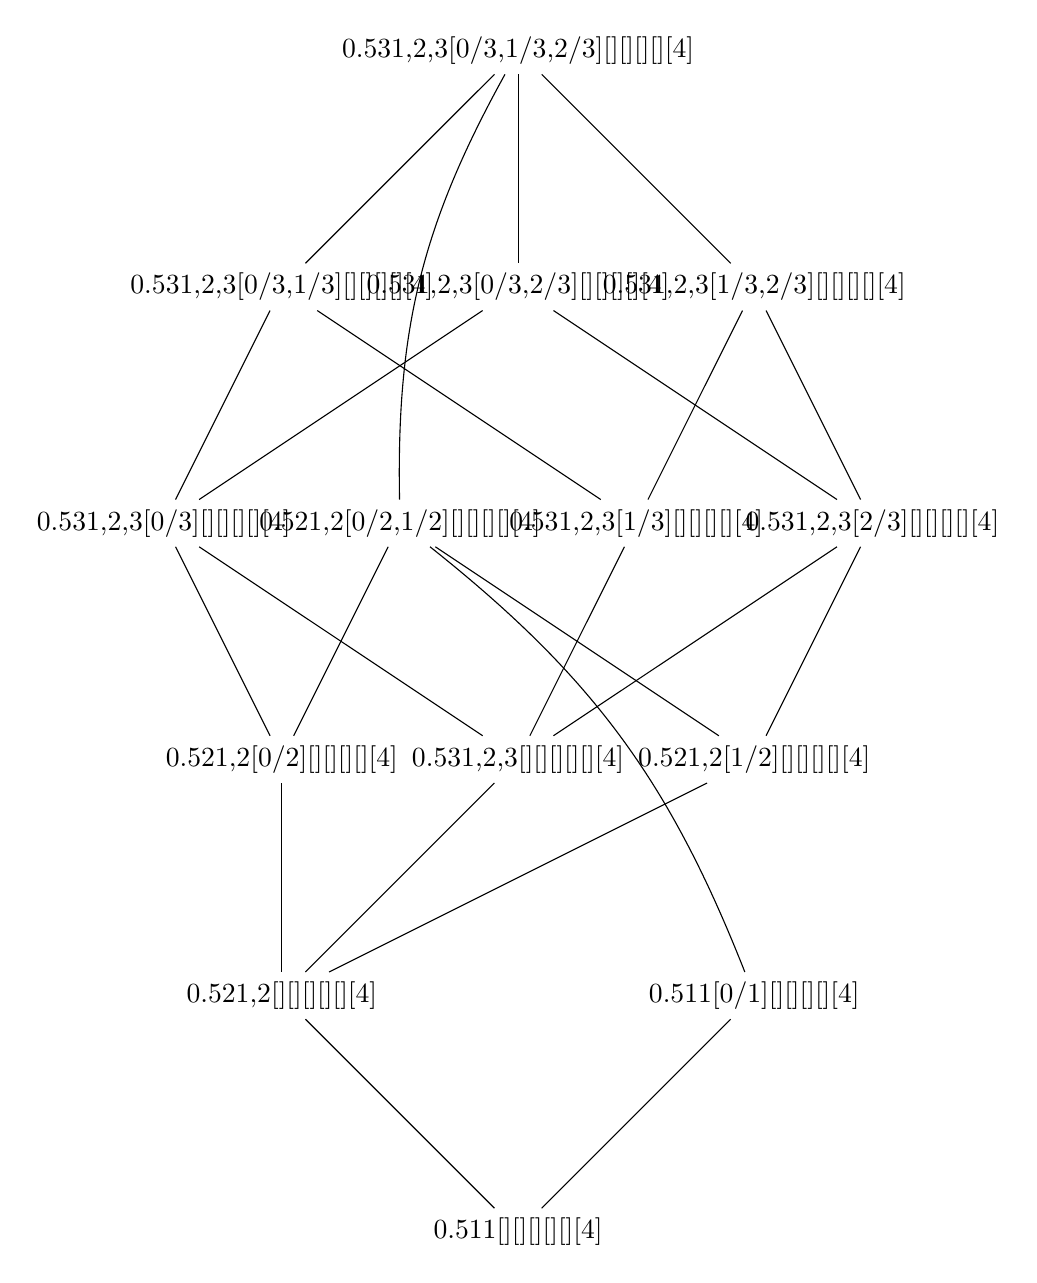
\begin{tikzpicture}
\def\y{3}
\def\x{3}
\def\s{0.5}
\node (123-123) at (0*\x,5*\y){\patt{\s}{3}{1,2,3}[0/3,1/3,2/3][][][][][4]};
\node (123-12) at (-1*\x,4*\y){\patt{\s}{3}{1,2,3}[0/3,1/3][][][][][4]};
\node (123-13) at (0*\x,4*\y){\patt{\s}{3}{1,2,3}[0/3,2/3][][][][][4]};
\node (123-23) at (1*\x,4*\y){\patt{\s}{3}{1,2,3}[1/3,2/3][][][][][4]};
\node (123-1) at (-1.5*\x,3*\y){\patt{\s}{3}{1,2,3}[0/3][][][][][4]};
\node (12-12) at (-0.5*\x,3*\y){\patt{\s}{2}{1,2}[0/2,1/2][][][][][4]};
\node (123-2) at (0.5*\x,3*\y){\patt{\s}{3}{1,2,3}[1/3][][][][][4]};
\node (123-3) at (1.5*\x,3*\y){\patt{\s}{3}{1,2,3}[2/3][][][][][4]};
\node (12-1) at (-1*\x,2*\y){\patt{\s}{2}{1,2}[0/2][][][][][4]};
\node (123-0) at (0*\x,2*\y){\patt{\s}{3}{1,2,3}[][][][][][4]};
\node (12-2) at (1*\x,2*\y){\patt{\s}{2}{1,2}[1/2][][][][][4]};
\node (12-0) at (-1*\x,1*\y){\patt{\s}{2}{1,2}[][][][][][4]};
\node (1-1) at (1*\x,1*\y){\patt{\s}{1}{1}[0/1][][][][][4]};
\node (1-0) at (0*\x,0*\y){\patt{\s}{1}{1}[][][][][][4]};
\draw (123-123) -- (123-12);\draw (123-123) -- (123-13);\draw (123-123) -- (123-23);
\draw[-] (123-123) to [bend right=15] (12-12);\draw[-] (12-12) to [bend left=15] (1-1);
\draw (123-12) -- (123-1);\draw (123-12) -- (123-2);
\draw (123-13) -- (123-1);\draw (123-13) -- (123-3);
\draw (123-23) -- (123-2);\draw (123-23) -- (123-3);
\draw (123-1) -- (123-0);\draw (123-1) -- (12-1);
\draw (123-2) -- (123-0);
\draw (123-3) -- (123-0);\draw (123-3) -- (12-2);
\draw (12-12) -- (12-1);\draw (12-12) -- (12-2);
\draw (12-1) -- (12-0);\draw (12-2) -- (12-0);
\draw (123-0) -- (12-0);\draw (12-0) -- (1-0);
\draw (1-1) -- (1-0);
\end{tikzpicture}
\caption{The interval $[1^\emptyset,123^{(0,3),(1,3),(2,3)}]$ of $\mathcal{M}$.}\label{fig:intEx}
\end{figure}

%
%Let $\pi_0=0$ and $\pi_{n+1}=n+1$ denote a imaginary points in the bottom left and top right corners, respectively. Given a set of points $B$ we say the area bounded by $B$ is boxes that lie between the leftmost and rightmost point and between the smallest and largest valued points. Moreover, given a box $(i,j)$, there is a unique set of points that bound that area $B(i,j)=\{\pi_i,\pi_{i+1},j,j+1\}$, which we call the \emph{bounding set} of $(i,j)$, denoted. Note these points might not be distinct so the set could have between $2$ and $4$ points.
%
%Given two mesh patterns $m$ and $p$ we define an \emph{occurrence} of $m$ in $p$ as an occurrence $\eta$ of $\cl(m)$ in $\cl(p)$ where a box $(i,j)$ is shaded in $m$ if and only if the area in $p$ bounded by the box $\{\eta(r)\,|\,r\in B(i,j)\}$ is fully shaded and contains no points.
%
%We can use this notion of occurrence to define a partial where $m\leM p$ if there is an occurrence of $m$ in $p$. Let $\mathcal{M}$ be the poset of all mesh patterns ordered by $\leM$. 
%
%The M\"obius function of a poset $Q$ is defined recursively by $\mu_Q(a,a)=1$ for all $a$, $\mu_Q(a,b)=0$ if $a\not\le b$ and if $a<b$ then:
%$$\mu_Q(a,b)=-\sum_{a\le c< b}\mu(a,c).$$
%When  it is clear which poset is being con
%
%A box $(i,j)$ can also be defined as the area $[i,i+1]\times[j,j+1]$. This box maps to the area $[\eta(i),\eta(i+1)]\times[\hat{\eta}(j),\hat{\eta}(j+1)]$ 
%
%An occurrence of $\sigma$ in $\pi$ is a map $\alpha:[|\sigma|]\rightarrow[|\pi|]$ such that $\alpha(1)\alph(2)\ldots\alpha(|\sigma|)$ has the same relative order of size. Given any letter $b=\sigma_i$ let $\hat{\alpha}(b)=\pi_{\alpha(i)}$, so $\hat{\alpha}$ maps the value of a letter to the value it has in the occurrence $\alpha$ in $\pi$.


\section{M\"obius Function}
We begin with some simple results we can immediately deduce about this poset. First we consider the case that two mesh patterns have the same underlying permutation.
\begin{lem}
If $\cl(m)=\cl(p)$, then $[m,p]$ is isomorphic to the boolean lattice $B_{|\sh(p)|-|\sh(m)|}$ which implies $\mu(m,p)=(-1)^|\sh(p)|-|\sh(m)|$ and $[m,p]$ is shellable.
\begin{proof}
We cannot remove any points from $p$, we can only unshade boxes, and we can unshaded any boxes from $\sh(p)\setminus\sh(s)$ in any order.
\end{proof}
\end{lem}

The simplest mesh patterns are those with no points, that is, the mesh patterns with a single box that is shaded or unshaded, which we denote $\epsilon^\emptyset$ and $\epsilon^{(0,0)}$, respectively.
\begin{lem}
Consider a mesh pattern $p$, then:
$$\mu(\epsilon^{A},p)=\begin{cases}
1,&\mbox{ if }p=\epsilon^A \\
-1,&\mbox{ if }A=\emptyset\,\,\&\,\,\rk(p)=1\\
0,&\mbox{ otherwise}
\end{cases}$$
\begin{proof}
The cases $p=\epsilon^A$ and $A=\emptyset\,\,\&\,\,\rk(p)=1$ are trivial. The mesh pattern $\epsilon^{(0,0)}$ is not contained in any large mesh patterns, so the M\"obius function is always $0$. If $\rk(p)>1$, then $(\epsilon^\emptyset,p)$ contains a unique minimal element $1^\emptyset$, so $\mu(\epsilon^\emptyset,p)$.
\end{proof}
\end{lem}

If two mesh patterns have no shadings then we have an interval from the classical poset.
\begin{lem}
If $\sh(s)=\sh(p)=\emptyset$, then $[s,p]$ is isomorphic to the interval $[\cl(s),\cl(p)]$ in $\mathcal{P}$, so $\muM(s,p)=\muP(\cl(s),\cl(p))$.
\end{lem}
The M\"obius function of the classical permutation poset is known to be unbounded \cite{Smith13}. So we get the following corollary:
\begin{cor}
The M\"obius function is unbounded on $\mathcal{M}$.
\end{cor}

We can also show that the M\"obius function is unbounded if we include shadings.
\begin{lem}\label{lem:mobUn}
Let $m$ be a mesh pattern with exactly one descent, where the descent bottom is the letter $1$, and all boxes south west of the point $1$ are shaded, then $$\mu(21^{(0,0),(1,0)},m)=\begin{cases}
(-1)^{|m|}\lfloor\frac{n}{2}\rfloor,&\mbox{ if } \cl(m) \mbox{ has no adjacencies}\\
1,&\substack{ \text{ if } \cl(m) \text{ has exactly one letter before the descent} \\\text{ in an adjacency tail and none after}}\\
0, &\mbox{ otherwise}
\end{cases}$$
Moreover, $[21^{(0,0),(1,0)},m]$ is shellable.
\begin{proof}
Note that every mesh pattern in $I=[21^{(0,0),(1,0)},m]$ has exactly one descent and everything SW of the point $1$ shaded. Define a bijection $f$ from $I$ to the poset of words with subword order where the $i-1$'th letter of $f(p)$ is $0$ if $i$ is before the letter $1$ in $p$ and $1$ if after the letter $1$, for all $1<i\le n$. So $21^{(0,0),(1,0)}$ maps to the word $0$. A mesh pattern in $I$ is uniquely determined by the value of the points before the descent, because these values must appear first followed by the letter $1$ and then the remaining letters. Therefore, it is straightforward to see this is a bijection and to check that it is order preserving. So $I$ is isomorphic to an interval of the poset of words with subword order. It was shown in \cite{Bjo90} that these intervals are shellable and the M\"obius function equals the number of normal occurrences, where an occurrence is normal if in any run of equal elements every non-initial letter is part of the occurrence, which implies the result.
\end{proof}
\end{lem}

We can also see that the M\"obius function on $\mathcal{M}$ is not bounded the classical poset, that is, it is not true that $\muM(m,p)\le \muP(\cl(m),\cl(p))$. A simple counterexample is the interval $[1^{(0,1)},123^{(0,2),(0,3),(1,2),(1,3)}]$, this has M\"obius number $1$, however $\muP(1,123)=0$.

If we consider intervals where the bottom mesh pattern has no shadings, then we get the following result:
\begin{lem}\label{lem:mu0}
Consider the interval $[m,p]$ in $\mathcal{M}$. If $\sh(m)=emptyset\not=\sh(p)$ and there is no $s\in(m,p)$ with $\cl(s)=\cl(m)$, then $\mu(m,p)=0$.
\begin{proof}
Define a map $f(x)=\cl(x)^\emptyset$, for any $x\in(m,p)$. Let $A$ order-preserving image $f((m,p))$. Note that $\mu(A)$ is contractible because it has a unique maximal element $\cl(p)^\emptyset$. Moreover, for any $y\in A$ $f^{-1}(A_{\ge y})$ equals $[y,p)$ which is contractible. Therefore, $(m,p)$ is homotopically equivalent to $A$ using the Quillen Fiber Lemma, which implies $\mu(m,p)=0$. This is also called a retraction.
\end{proof}
%\begin{proof}
%Define a map the maps the mesh pattern to the mesh pattern with no shadings. This is well defined in this case because there are no shadings of $\sigma$ in $\pi$ so the image of the map from $(\sigma,\pi)$ is contained in $(\sigma,\pi)$. There will be a cone point of $cl(\pi)^\emptyset$, so the image is contractible. Moreover, each fibre is contractible because $f^{-1}(Q_\ge x)$ will all contain $x$.
%\end{proof}
\end{lem}
We can combine Lemma~\ref{lem:mu0} with he following result to see that the M\"obius function is almost always zero on the interval $[1^\emptyset,p]$.
\begin{lem}
As $n$ tends to infinity the proportion of permutations that contain one of $\{1^{(0,0)},1^{(1,0)},1^{(0,1)},1^{(1,1)}\}$ approaches $0$.
\begin{proof}
Let $P(n,i)$ be the probability that the letter $i$ is an occurrence of $1^{(0,0)}$ in a length $n$ mesh pattern. And let $P(n)$ be the probability that a length $n$ mesh pattern contains $1^{(0,0)}$.

The probability that $i$ is an occurrence of $1^{(0,0)}$ is given by selecting the location $k$ of $i$, each has probability $\frac{1}{n}$, and then we require that all boxes south west of $i$ are filled, of which there are $2^{ik}$. Note that this over estimates the probability, because it is possible that there is a point south west of $i$, which would imply $i$ is not an occurrence of $1^{(0,0)}$, however this argument still counts them. We can formulate this as:
\begin{align*}
P(n,i)&\le\sum_{k=1}^{n+1-i}\frac{1}{n}\left(\frac{1}{2^i}\right)^k=\frac{1}{n}\left(\frac{2^{-i(n+2-i)}}{2^{-i}-1}-1\right)=\frac{1}{n2^i}\left(\frac{1-2^{-i(n+1-i)}}{1-2^{-i}}\right)\le\frac{2}{n2^i}
\end{align*}

To compute the probability that a length $n$ permutation contains $1^{(0,0)}$ we can sum over all letters $i$ and test if $i$ is an occurrence of $1^{(0,0)}$. Note again this is an over estimate because if a permutation contains multiple occurrences of $1^{(0,0)}$ it counts that permutation more than once.

$$P(n)\le\sum_{i=1}^{n}P(n,i)\le\sum_{i=1}^{n}\frac{2}{n2^i}=\frac{2}{n}\left(\frac{\left(\frac{1}{2}\right)^{n+1}-1}{\frac{1}{2}-1}-1\right)\le\frac{2}{n} $$

We can repeat this calculation for the other three one shadings of $1$ so we get that $P(n)\le \frac{4}{n}\rightarrow 0$.
\end{proof}
\end{lem}
\begin{cor}
As $n$ tends to infinity the proportion of mesh patterns $p$ of length n such that $\mu(1^\emptyset,p)=0$ approaches $1$.
\end{cor}


In the classical case it is true that given a permutation $\sigma$ the probability a permutation of length $n$ contains $\sigma$ tends to $1$ as $n$ tends to infinity, this follows from the Marcus-Tardos Theorem \cite{MT04}. By the above result we can see the same is not true in the mesh pattern case. In fact we conjecture the opposite is true:
\begin{conj}
Given a mesh pattern $m$, the probability that a random mesh pattern of length $n$ contains $m$ tends to $0$ as $n$ tends to infinity.
\end{conj}




\section{Purity}

Interestingly the mesh pattern poset is not a pure poset, that is, not every maximal chain has the same length. We say an edge $x\lessdot y$ is \emph{impure} if $\rk(y)-\rk(x)>1$. Let $m-p$ be the mesh pattern obtained by deleting the point $p$ and let $m\setminus p$ be the occurrence of $m-p$ in $m$. We say that deleting a point $p$ \emph{merges shadings} if there is a shaded box in $m-p$ that corresponds to more than $1$ shaded box in $m\setminus p$.

\begin{lem}\label{lem:impureEdge}
An edge between $x\lessdot y$ is impure if and only if all occurrences of $x$ in $y$ use all shaded boxes of $y$ and are obtained by deleting a point that merges shading.
\begin{proof}
First we show the backwards direction. Because $x$ is obtained by deleting a point that merges shadings $x$ must have one less point and at least one less shading so $\rk(y)-\rk(x)\ge2$. So it suffices to show that there is no $z$ such that $x<z<y$. Suppose such a $z$ exists, then if $z$ is obtained by deshading a box in $y$ it can no longer contain $x$ because all occurrences of $x$ in $y$ use all shaded areas of $y$. If $z$ is obtained by deleting a point, then that cannot remove shadings, only merge shadings, otherwise it wouldn't contain $x$, and it implies $cl(x)=cl(z)$. Moreover, if $x<z$ then we can deshade some boxes of $z$ to get $x$ which implies there is an occurrence of $x$ in $y$ that doesn't use all the shaded boxes of $y$.

Now consider the forwards direction, so suppose $x\lessdot y$ is impure. So $\rk(y)-\rk(x)\ge2$, which implies $x$ is obtained by deleting a single point which merges shadings but does not delete shadings, because any other combination of deleting points and deshading can be done in successive steps. Furthermore, this must be true for any point that can be deleted to get $x$, that is, for all occurrences of $x$ in $y$. Moreover, if there is an occurrence that doesn't use all the shaded boxes of $y$, we can deshade the box it doesn't use and get an element that lies between $x$ and $y$.
\end{proof} 
\end{lem}

\begin{lem}\label{lem:topImpure}
If there is an impure edge in $[1^\emptyset,m]$, then there is an impure edge $a\lessdot b$ where $cl(m)=cl(b)$.
\begin{proof}
If $x\lessdot y$ is an impure edge in $[1^\emptyset,m]$, then let $b$ be a mesh pattern obtained by adding points to $y$ to get the classical pattern $b$. Pick an occurrence of $x$ in $y$ and add the points to $x$ in the order induced by how they are added to $y$ and the occurrence, call this $a$. The points added will not have any shadings in the four boxes touching it, therefore no point touching a shading in $a$ can embed in a new point of $b$. Moreover, the set of embeddings of $a$ in $b$ is a subset of $x$ in $y$, after adding the new points to each. These two conditions imply that if every embedding of $x$ in $y$ uses all the shadings of $y$, this is also true for every embedding of $a$ in $b$. Therefore, the result follows by Lemma~\ref{lem:impureEdge}.
\end{proof}
\end{lem}

\begin{prop}
Consider a mesh pattern $m$. The interval $[1^\emptyset,m]$ is non-pure if and only if there exists a point $p$ in $m$ such that $m-p$ merges shadings and there is no other occurrence of $m-p$ in $m$ with a subset of shadings of $m\setminus p$.
\begin{proof}
First we show the backwards direction. Let $x$  be the mesh pattern obtained by inserting $p$ back into $m^p$, and $\eta$ the corresponding embedding of $m^p$ in $x$. Note that it is not always true that $x=m$ because some shaded shadings of $m$ are lost when deleting $p$. We claim that $m^p\lessdot x$ is an impure edge. This follows by Lemma~\ref{lem:impureEdge} because by $\eta$ uses all the shaded boxes in $x$ and there is no subshading occurrence.

To see the other direction suppose there is an impure edge in $[\omega,m]$. By Lemma~\ref{lem:topImpure} there is an impure edge $a\lessdot b$ where $cl(b)=cl(m)$. If $m$ is impure then it must remove both a point and a shading, so it must merge shadings by deleting some point $p$ and there is no element between them so there can be no subshading of $b$ that contains $a$.
\end{proof}
\end{prop}

\begin{cor}
There is an impure edge in the interval $[m,p]$ if and only if there exists a point $x$ in $p$ such that $p-x$ merges shadings and there is no other occurrence of $p-x$ in $p$ with a subset of shadings of $p\setminus x$, and $p-x\ge m$.
\end{cor}

Note that containing an impure edge in $[m,p]$ does not necessarily imply there that $[m,p]$ is non-pure. For example, if $[m,p]$ contains only one edge and that edge is impure, then $[m,p]$ is still pure. So it is necessary that there is an impure edge and a pure edge in the interval. Although it is also possible to have an non-pure poset that only contains impure edges, if the difference between the ranks of the elements at ends of the edges varies.


\section{Topology}

If $[\cl(s),\cl(p)]$ is (dis)connected in $\mathcal{P}$ it does no imply $[s,p]$ has the same property in $\mathcal{M}$. For example, the interval $[123,456123]$ is disconnected in the classical permutation poset but in $\mathcal{M}$ the interval $[123^{(3,0),(3,1),(3,2)},456123^{(6,0),(6,1),(6,2)}]$, see \cref{fig:123}, is chain, so is connected. Furthermore, the interval $[321,521643]$ is connected in $\mathcal{P}$ but $[321^{(1, 3)},521643^{(1, 5), (1, 6), (4, 6)}]$, see \cref{fig:321}, is disconnected in $\mathcal{M}$.
\begin{figure}[h]\centering
\patt{.5}{3}{1,2,3}[3/0,3/1,3/2][][][][][4]
\patt{.5}{6}{4,5,6,1,2,3}[6/0,6/1,6/2][][][][][4]
\caption{The mesh patterns $123^{(3,0),(3,1),(3,2)}$ and $456123^{(6,0),(6,1),(6,2)}$}\label{fig:123}
\end{figure}
\begin{figure}[h]\centering
\patt{.5}{3}{3,2,1}[1/3][][][][][4]
\patt{.5}{6}{5,2,1,6,4,3}[1/5,1/6,4/6][][][][][4]
\caption{The mesh patterns $321^{(1, 3)}$ and $521643^{(1, 5), (1, 6), (4, 6)}$}\label{fig:321}
\end{figure}

This also implies that if $[\cl(s),\cl(p)]$ is (non-)shellable in $\mathcal{P}$ then it is not true that $[s,p]$ has the same property in $\mathcal{M}$. This follows by the previous examples, $[123,456123]$ is not shellable but $[123^{(3,0),(3,1),(3,2)},456123^{(6,0),(6,1),(6,2)}]$ is shellable, and $[321,521643]$ is shellable but $[321^{(1, 3)},521643^{(1, 5), (1, 6), (4, 6)}]$ is not shellable.

We can define a direct sum operation on mesh patterns, where given two mesh patterns $s$ and $t$, where the top right corner of $s$ and bottom left corner of $t$ are not shaded, the direct sum $s\oplus t$ has classical pattern $\cl(s)\oplus\cl(t)$ and the shadings are given by placing $t$ north east of $s$ and shading any borders so they extend to the edge. We can similarly define the skew-sum.

\begin{lem}
If $m$ is indecomposable and $(0,0),(|m|,|m|)\not\in\sh(m)$, then $[m,m\oplus m]$ is disconnected.
\begin{proof}
There are exactly two occurrences of $m$ in $m\oplus m$, the first $|m|$ letters $\eta_1$ or the last $|m|$ letters $\eta_2$. If you delete a point or deshade any box that is not in $\eta_1$ then that point or box must be part of $\eta_2$, so the resulting mesh pattern only contains one occurrence of $m$ which corresponds to $\eta_1$ so then you can only delete points or shadings that are not part of $\eta_1$ so must be part of $\eta_2$. A similar argument applies if you initial delete a point or shading not part of $\eta_2$. Therefore, any two points/shading removals must both be part of $\eta_1$ or $\eta_2$, thus the poset can be split into components where on one side we remove elements not in $\eta_1$ and the other elements not in $\eta_2$.
\end{proof}
\end{lem}
\begin{cor}
If $m$ is indecomposable and $(|m|,0),(0,|m|)\not\in\sh(m)$, then $[m,m\ominus m]$ is disconnected.
\end{cor}

A analogous result is used in the classical case in \cite{McSt13} to show that almost all intervals of the classical permutation poset are not shellable. The proof of this follows form the Marcus-Tardos theorem, we have seen this result does not apply in the mesh pattern case so we cannot prove a similar result using this technique.  A similar problem was studied for boxed mesh patterns in permutations in \cite{AKV13}, which is equivalent to boxed mesh patterns in fully shaded mesh patterns. So we leave it as an open question
\begin{que}
What proportion of intervals of $\mathcal{M}$ are shellable?
\end{que}

\iffalse

\section{Results: Sketch}
Consider the Mesh pattern poset $\mathcal{M}$. Given a mesh pattern $p=(\pi,P)$ we let $\cl(p)=\pi$ and $\sh(p)=P$, we also use the notation $p=\pi^P$ to represent the mesh pattern. We let $|\pi|$ represent the length of $\pi$ and $|P|$ the size of $P$. We define the \emph{rank} of $p$ as $|\pi|+|P|$, that is, the number of points plus the number of shaded boxes. We define the length of $p$ as $|p|=|\pi|$, that is, the number of points. We use $\muP$ to denote the M\"obius function in the classical permutation poset $\mathcal{P}$ and $\muM$, or just $\mu$ when unambiguous, to denote the M\"obius function in the Mesh pattern poset.

\begin{lem}
Consider two mesh patterns $[s,p]$:
\begin{itemize}
\item If $\cl(s)=\cl(p)$, then $[s,p]$ is isomorphic to the boolean lattice $B_{|\sh(p)|-|\sh(s)|}$ which implies $\mu(s,p)=(-1)^|\sh(p)|-|\sh(s)|$.
\item If $\sh(s)=\sh(p)=\emptyset$, then $[s,p]$ is isomorphic to the interval $[\cl(s),\cl(p)]$ in the classical permutation poset, so $\muM(s,p)=\muP(\cl(s),\cl(p))$.
\item If $\rk(s)=0$, that is, $s$ is the empty mesh pattern, then $\mu(s,m)=0$ for every $m$ with $\rk(m)>1$.
\end{itemize}
\end{lem}

Because the M\"obius function is unbounded on $\mathcal{P}$ and all intervals of $\mathcal{P}$ are in $\mathcal{M}$ we know that:
\begin{cor}
The M\"obius function is unbounded on $\mathcal{M}$.
\end{cor}

If we add shadings as well then we still get an unbounded M\"obius function:
\begin{lem}
Let $m$ be a mesh pattern with exactly one descent, where the descent bottom is the letter $1$, and all boxes south west of the point $1$ are shaded, then $$\mu(21^{(0,0),(1,0)},m)=\begin{cases}
(-1)^{|m|}\lfloor\frac{n}{2}\rfloor,&\mbox{ if } \cl(m) \mbox{ has no adjacencies}\\
1,&\mbox{ if } \cl(m) \mbox{ has exactly one adjacency tail letter before the descent and none after}\\
0, &\mbox{ otherwise}
\end{cases}$$
Moreover, $[21^{(0,0),(1,0)},m]$ is shellable.
\end{lem}

We can also consider these intervals starting at the mesh pattern $21^\emptyset$:
\begin{lem} There is a problem here, in that the image of any element with underlying perm is going to map to $\cl(m)$ which is not in $(mu(21^{(0,0),(1,0)},m)$. For example consider $m=213^{(0,0),(1,0)}$.

If $m$ is mesh pattern with all boxes south west of the point $1$ shaded, then $\mu(21^emptyset,m)=\mu(21^{(0,0),(1,0)},m)$. Moreover, $[21^emptyset,m]$ is CM if and only if $[mu(21^{(0,0),(1,0)},m]$ is CM.
%\begin{proof}
%Define a map from $(21^epsilon,m)$ which maps an element $x$ to $(21^{(0,0),(1,0)},m)$ by filling all boxes south west of $1$ in $x$. Because $21^{(0,0),(1,0)}$ is not in $(21^{(0,0),(1,0)},m)$ we deal with it as a special case where you pick any element $\lambda$ of rank $3$ and map elements with classical pattern $21$ to $\lambda$. Every element not $\lambda$ has a unique bottom element in it's fibre, the element with $cl(\lambda)$ with no shadings. Moreover, the fibre of $\lambda$ has 3 bottom elements the one with no shading and the two 1 box shadings of $21$, the two $1$ box shadings are contained in a single element of rank 1 high, that obtained by shading the leftmost or right most box of the south west corner, so these points can be contracted, so the fibre is again contractible. The result then follows by the Quillen fibre lemma.
%\end{proof}
\end{lem}

It is not true that the M\"obius function of an interval $[s,m]$ is bounded by $\muP(\cl(s),\cl(m))$. For a counter example consider $[1^{(0,1)},123^{(0,2),(0,3),(1,2),(1,3)}]$ this has M\"obius number $1$ but $\muP(1,123)=0$.

The M\"obius function of almost all intervals $[1^\emptyset,m]$ equals $0$. We can see this using the following results:
\begin{lem}
If $\sh(s)=emptyset$ and there is no $\lambda\in(s,p)$ with $\cl(\lambda)=\cl(s)$, then $\mu(s,p)=0$.
%\begin{proof}
%Define a map the maps the mesh pattern to the mesh pattern with no shadings. This is well defined in this case because there are no shadings of $\sigma$ in $\pi$ so the image of the map from $(\sigma,\pi)$ is contained in $(\sigma,\pi)$. There will be a cone point of $cl(\pi)^\emptyset$, so the image is contractible. Moreover, each fibre is contractible because $f^{-1}(Q_\ge x)$ will all contain $x$.
%\end{proof}
\end{lem}

\begin{cor}
If $m$ has no point where everything NE, NW, SE or SW is shaded then $\mu(1^\emptyset,m)=0$.
\end{cor}

We can generalise this result slightly:
\begin{lem}I think the conditions on this need to be stricter, something like if $\lambda<t$ then for any classical perm $r\in[\cl(t),\cl(p)]$ there is a mesh $q\in[\lambda,p)$ with $\cl(q)=r$.

Consider $[s,p]$, where $\sh(s)=\emptyset\not=\sh(p)$. If for every $\lambda\in(\sigma,\pi)$ with $\cl(\lambda)=\cl(s)$ there is a $\tau\in(s,p)$ with $\cl(\tau)=\cl(p)$ and $\lambda\le\tau$, then $\mu(s,p)=0$.
%\begin{proof}
%Define a map the maps the mesh pattern to the mesh pattern with no shadings. This is well defined in this case because there are no shadings of $\sigma$ in $\pi$ so the image of the map from $(\sigma,\pi)$ is contained in $(\sigma,\pi)$. There will be a cone point of $cl(\pi)^\emptyset$, so the image is contractible. Moreover, each fibre is contractible because $f^{-1}(Q_\ge x)$ will all contain $x$.
%\end{proof}
\end{lem}

\begin{lem}I think the conditions on this need to be stricter, something like if $\lambda<t$ then for any classical perm $r\in[\cl(t),\cl(p)]$ there is a mesh $q\in[\lambda,p)$ with $\cl(q)=r$.

Consider $[s,p]$, where $\sh(s)=\emptyset\not=\sh(p)$. If for every $\lambda\in(\sigma,\pi)$ with $\cl(\lambda)=\cl(s)$ there is a $\tau\in(s,p)$ with $\cl(\tau)=\cl(p)$ and $\lambda\le\tau$, then $[s,p]$ is CM if and only if $[\cl(s),\cl(p)]$ is CM.
%\begin{proof}
%By the map we defined before $(\sigma,\pi)$ is homotopically equivalent to $(cl(\sigma),cl(\pi)]$, which is a coning of $(cl(\sigma),cl(\pi))$, so is CM if and only if $[(cl(\sigma),cl(\pi)]$ is CM.
%\end{proof}
\end{lem}

Interestingly the Mesh pattern poset is not a pure poset, that is, not every maximal chain has the same length. We say an edge $x\lessdot y$ is \emph{impure} if $\rk(y)-\rk(x)>1$. Let $m-p$ be the mesh pattern obtained by deleting the point $p$ and let $m\setminus p$ be the occurrence of $m-p$ in $m$. We say that deleting a point $p$ \emph{merges shadings} if there is a shaded box in $m-p$ that corresponds to more than $1$ shaded box in $m\setminus p$.

\begin{lem}\label{lem:impureEdge}
An edge between $x\lessdot y$ is impure if and only if all occurrences of $x$ in $y$ use all shaded boxes of $y$ and are obtained by deleting a point that merges shading.
%\begin{proof}
%First we show the backwards direction. Because $x$ is obtained by deleting an point that merges shadings $x$ must have one less point and at least one less shading so $\rk(y)-\rk(x)\ge2$. So it suffices to show that there is no $z$ such that $x<z y$. Suppose such a $z$ exists then if $z$ is obtained by deshading a box in $y$ it can no longer contain $x$ because all occurrences of $x$ in $y$ use all shaded areas of $y$. If $z$ is obtained by deleting a point then that cannot remove shadings only merge, otherwise it wouldn't contain $x$, and it implies $cl(x)=cl(z)$ and if $x<z$ then we can deshade some boxes of $z$ to get $x$ which implies there is an occurrence of $x$ in $y$ that doesn't use all the shaded boxes of $y$.
%
%To show the other direction. Because $\rk(y)-\rk(x)\ge2$, then $x$ is obtained by deleting a point and merge some shadings, because any other combination or removing more than one element can be done in succesive steps. Furthermore, this must be true for all occurrences of $x$ in $y$ otherwise there will be an alternative pure route through the occurrences that doesn't have this. Moreover, if there is an occurrence that doesn't use all the shaded boxes of $y$, we can deshade the box it doesn't use and get an element that lies between $x$ and $y$.
%\end{proof} 
\end{lem}

\begin{lem}\label{lem:topImpure}
If there is an impure edge in $[1^\emptyset,m]$, then there is an impure edge $a\lessdot b$ where $cl(m)=cl(b)$.
%\begin{proof}
%[Not fully convinced by proof]If $x\lessdot y$ is an impure edge in $[\omega,m]$ then let $b$ be a mesh pattern obtained by adding points to $y$ to get the classical pattern $b$. Pick an occurrence of $x$ in $y$ and add the points to $x$ in the order induced by how they are added to $y$ and the occurrence, call this $a$. The points added will not have any shadings in the four boxes touching it, therefore no point touching a shading in $a$ can embed in a new point of $b$. Moreover, the set of embeddings of $a$ in $b$ is a subset of $x$ in $y$, after adding the new points to each. These two conditions imply that if every embedding of $x$ in $y$ uses all the shadings of $y$, this is also true for every embedding of $a$ in $b$. Therefore, the result follows by Lemma~\ref{lem:impureEdge}.
%\end{proof}
\end{lem}

\begin{prop}
Consider a mesh pattern $m$. The interval $[1^\emptyset,m]$ is non-pure if and only if there exists a point $p$ in $m$ such that $m-p$ merges shadings and there is no other occurrence of $m-p$ in $m$ with a subset of shadings of $m\setminus p$.
%\begin{proof}
%First we show the backwards direction. Let $x$  be the mesh pattern obtained by inserting $p$ back into $m^p$, and $\eta$ the corresponding embedding of $m^p$ in $x$. Note that it is not always true that $x=m$ because some shaded shadings of $m$ are lost when deleting $p$. We claim that $m^p\lessdot x$ is an impure edge. This follows by Lemma~\ref{lem:impureEdge} because by $\eta$ uses all the shaded boxes in $x$ and there is no subshading occurrence.
%
%To see the other direction suppose there is an impure edge in $[\omega,m]$. By Lemma~\ref{lem:topImpure} there is an impure edge $a\lessdot b$ where $cl(b)=cl(m)$. If $m$ is impure then it must remove both a point and a shading, so it must merge shadings by deleting some point $p$ and there is no element between them so there can be no subshading of $b$ that contains $a$.
%\end{proof}
\end{prop}

If $[\cl(s),\cl(p)]$ is (dis)connected in $\mathcal{P}$ it does no imply $[s,p]$ has the same property in $\mathcal{M}$. For example, the interval $[123,456123]$ is disconnected in $\mathcal{P}$ but $[123^{(3,0),(3,1),(3,2)},456123^{(6,0),(6,1),(6,2)}]$ is chain, so is connected. Furthermore, the interval $[321,521643]$ is connected in $\mathcal{P}$ but $[321^{(1, 3)},521643^{(1, 5), (1, 6), (4, 6)}]$ is disconnected in $\mathcal{M}$.

This also implies that if $[\cl(s),\cl(p)]$ is (non-)shellable in $\mathcal{P}$ then it is not true that $[s,p]$ has the same property in $\mathcal{M}$. This follows by the previous examples, $[123,456123]$ is not shellable but $[123^{(3,0),(3,1),(3,2)},456123^{(6,0),(6,1),(6,2)}]$ is shellable, and $[321,521643]$ is shellable but $[321^{(1, 3)},521643^{(1, 5), (1, 6), (4, 6)}]$ is not shellable.

We can define a direct sum operation on mesh patterns, where given two mesh patterns $s$ and $t$, where the top right corner of $s$ and bottom left corner of $t$ are not shaded, the direct sum $s\oplus t$ has classical pattern $\cl(s)\oplus\cl(t)$ and the shadings are given by placing $t$ north east of $s$ and shading any borders so the extend to the edge.

\begin{lem}
If $s$ is indecomposable, then $[s,s\oplus s]$ is disconnected.
\end{lem}

\begin{conj}
Almost every interval of $\mathcal{M}$ is not shellable.
%\begin{proof}
%This should follow by a similar proof to that used in the classical case by Peter and Einar. Although the fact that you require two opposite corners of the mesh pattern to be unshaded may make it more difficult. i think only $\frac{7}{16}$ of mesh pattern will have two opposite corners unshaded.
%\end{proof}
\end{conj}

\begin{lem}
If there is a unique minimal shading $x\in(s,p)$ of $p$, and a unique minimal shading of every element $\lambda\in(s,p)$ contained in $x$, then $\mu(s,p)=0$. 
\end{lem}

\begin{lem}
If $\cl(s)$ and $\cl(p)$ begin with $1$ and the leftmost column is fully shaded in both $s$ and $p$, with no other shadings, then $\mu(s,p)=\mu(\cl(s)_{>1},\cl(p)_{>1})$.
\end{lem}

\fi
	
\iffalse

My definition of normal doesn't work. Consider $[21^\emptyset,231^{(1, 0), (0, 0)}]$ it has 1 normal embedding according to my definition but the mob is $0$.

If for every classical pattern $\lambda$ in $(s,p)$ there is a unique minimal shading of $\lambda$ in $(s,p)$, and at least one element with $cl(p)$ in $(s,p)$, then $\mu(s,p)=0$.

If there is a unique minimal shading of $p$ that is in $(s,p)$, and every element $\lambda\in(s,p)$ is contained in some $\pi\in(s,p)$ with $\cl(\pi)=\cl(p)$, then $\mu(s,p)=0$. 

If there is a unique minimal shading $x\in(s,p)$ of $p$, and every element $\lambda\in(s,p)$ is contained in some $\pi\in(s,p)$ with $\cl(\pi)=\cl(p)$ or there is a unique minimal shading of $\lambda$ contained in $x$, then $\mu(s,p)=0$.


If for every classical pattern $\lambda$ in $(s,p)$ there is a unique maximal shading of $\lambda$ in $(s,p)$, and at least on element with $cl(s)$ in $(s,p)$, then $\mu(s,p)=0$.








Let $M$ be the poset of all mesh patterns. Let $P$ be the classical permutation poset. Unless otherwise stated $\mu=\mu_M$. Let $\omega$ be the mesh pattern with a single point and no shading. Given a mesh pattern $m$ let $m^p$ be the permutation and $m^s$ the shading.

\begin{lem}
Consider two mesh patterns $[s,m]$. If $s^p=m^p$, then $[s,m]$ is isomorphic to a boolean lattice. If $m^s$ is empty then $[s,m]$ is isomorphic to $[s^p,m^p]$ in $P$.  
\end{lem}
	
\begin{cor}
The M\"obius function is unbounded on $M$.
\begin{proof}
This follows because the M\"obius function on $P$ is unbounded.
\end{proof}
\end{cor}

Let $t$ be the mesh pattern on $12$ with the right two cells on the top row shaded. We know that intervals of $M$ are not necessarily pure because $[\omega,t]$ is not. Also $[\omega,t]$ is disconnected, so not shellable. By computation we now give a mesh pattern $x$ on $12$, the interval $[\omega,x]$ is pure if and only if $x$ does not contain $t$.

\begin{conj}
Given a mesh pattern pair $s$, $m$, if $|m^s|=1$, $|s^s|=0$ and $\rk(s,m)>2$, then $\mu(\omega,m)=0$.
\end{conj}

\begin{conj}
Consider a mesh pattern $m$, if there is a point such that all cells east or west on the lines above or below are filled or similar all cells north or south on the column left or right are filled, then $[\omega,m]$ is nonpure.
\end{conj}
The above conjecture does not hold in the other direction.
%here is a counterexample MeshPatt(Perm((0, 2, 1, 4, 3, 5, 6)), frozenset({(4, 1), (4, 3), (4, 0)}))


If $[\omega,m]$ is non-pure then there must be a pair of consecutive shaded cells in $m$. Again this the other direction doesn't hold.

\begin{conj}
The interval $[\omega,m]$ is pure if and only if there is a point such that every shaded cell in it's cross is part of a pair and deleting that point gives an element for which there is no other occurrence of in $m$ that can be obtained by not deleting a cell with shadings in the cross
\end{conj}

\begin{conj}
If $m$ is a mesh pattern on an increasing perm, then $[\omega,m]$ is pure if and only if in every line from a point of the perm has the first and last element shaded, which are not equal, at least two consecutive shaded points and no two consecutive non-shaded points. 
\end{conj}

A line from a point refers to the single row or column extend out from a point of the perm.

\begin{conj}NOT TRUE
Consider a mesh pattern $m$, the interval $[\omega,m]$ is nonpure if and only if for any adjacency in $m$ there is a corresponding sequence on filled squares in a row or column that covers the whole adjacency or touches a point of the adjacency and covers everything upto that point.
\end{conj}


Given any mesh pattern $m$ and a mesh pattern $n$ with no shadings in $n$ then $\rk(\omega,m)$ equals the length of the pattern in $m$ plus the number of shaded squares minus the length of $n$. However if you allow the bottom element to have shaded squares this doesn't hold, to see an example take any edge that is impure so between different ranked elements and make the poset with just that edge.

\begin{conj}FALSE (MIGHT BE BOUNDED BY 1 THOUGH)
If $n$ has no shadings and $m$ has shadings, then 
$$\mu(n,m)=\begin{cases}(-1)^{|m^s|},&\mbox{ if }n^p=m^p\\0,&\mbox{ otherwise}\end{cases}$$
\begin{proof}
The case $n^p=m^p$ follows by the fact the interval is a boolean lattice. To show the other cases probably follows by some kind of inductive argument on the dual of $\mu$ where all nonzero mob valued elements contain the pattern obtained by unshading all boxes of $m$.
\end{proof}
\end{conj}

\begin{conj}
Almost all intervals $[\omega,m]$ are impure
\end{conj}
\begin{conj}
Almost all intervals have Mobius number 0.
\end{conj}

The M\"obius function is not bounded by 1, take the interval [21,2413] and shade the left most cells in the top row of 2413, this has mob $-2$

\begin{conj}
An edge $\sigma\lessdot\pi$ is impure in $[\omega,\pi]$ if and only if there is exactly one occurrence of $\sigma$ in $\pi$ and $\sigma$ is obtained from $\pi$ by deleting a single point that merges at least one pair of shaded boxes.
\begin{proof}
You must delete  point such that  a pair of shaded boxes merges in order to go down more than one rank, the exactly one occurrence condition ensures that there is no point between $\sigma$ and $\pi$. If there is more than one occurrence than you can remove empty shaded boxes from one occurrences and then delete the appropriate letter and which creates element between.
\end{proof}
\end{conj}

I think, we can test if a interval if impure by looking for two shaded boxes next to each other split by a point, not touching, remove any single points in the cross, and see if removing that point gives an element with only one occurrence in the top mesh.

This works on the conjecture that if the interval is impure there is an impure edge from a mesh pattern with the same underlying permutation.

I think the condition is not exactly one occurrence, but exactly one occurrence of the shadings. So we treat two occurrences as the same if they give the same shaded areas, and there is at least one shading.

We say that two embeddings $\sigma$ in $\pi$ are equivalent if the shaded areas of $\sigma$ correspond to the same areas in $\pi$ in both embeddings.

That's also not it, I think it might be that the pairs of cells that merge must overlap for all the occurrences (and for all pairs that merge)

We say an occurrence of $\sigma$ in $\pi$ \emph{merges boxes} if at least one shaded box in $\sigma$ corresponds to more that one box in $\pi$.



\begin{lem}\label{lem:impureEdge}
An edge between $x\lessdot y$ is impure if and only if all occurrences of $x$ in $y$ use all shaded boxes of $y$ and are obtained by deleting a point that merges shading.
\begin{proof}
First we show the backwards direction. Because $x$ is obtained by deleting an point that merges shadings $x$ must have one less point and at least one less shading so $\rk(y)-\rk(x)\ge2$. So it suffices to show that there is no $z$ such that $x<z y$. Suppose such a $z$ exists then if $z$ is obtained by deshading a box in $y$ it can no longer contain $x$ because all occurrences of $x$ in $y$ use all shaded areas of $y$. If $z$ is obtained by deleting a point then that cannot remove shadings only merge, otherwise it wouldn't contain $x$, and it implies $cl(x)=cl(z)$ and if $x<z$ then we can deshade some boxes of $z$ to get $x$ which implies there is an occurrence of $x$ in $y$ that doesn't use all the shaded boxes of $y$.

To show the other direction. Because $\rk(y)-\rk(x)\ge2$, then $x$ is obtained by deleting a point and merge some shadings, because any other combination or removing more than one element can be done in succesive steps. Furthermore, this must be true for all occurrences of $x$ in $y$ otherwise there will be an alternative pure route through the occurrences that doesn't have this. Moreover, if there is an occurrence that doesn't use all the shaded boxes of $y$, we can deshade the box it doesn't use and get an element that lies between $x$ and $y$.
\end{proof} 
\end{lem}

\begin{lem}[Not fully convinced by proof]\label{lem:topImpure}
If there is an impure edge in $[\omega,m]$ then there is an impure edge $a\lessdot b$ where $cl(m)=cl(b)$.
\begin{proof}
If $x\lessdot y$ is an impure edge in $[\omega,m]$ then let $b$ be a mesh pattern obtained by adding points to $y$ to get the classical pattern $b$. Pick an occurrence of $x$ in $y$ and add the points to $x$ in the order induced by how they are added to $y$ and the occurrence, call this $a$. The points added will not have any shadings in the four boxes touching it, therefore no point touching a shading in $a$ can embed in a new point of $b$. Moreover, the set of embeddings of $a$ in $b$ is a subset of $x$ in $y$, after adding the new points to each. These two conditions imply that if every embedding of $x$ in $y$ uses all the shadings of $y$, this is also true for every embedding of $a$ in $b$. Therefore, the result follows by Lemma~\ref{lem:impureEdge}.
\end{proof}
\end{lem}

\begin{prop}
Consider a mesh pattern $m$. The interval $[\omega,m]$ is nonpure if and only if there exists a point $p$ in $m$ such that deleting $p$ merges shadings, giving $m^p$, and there is no other occurrence of $m^p$ in $p$ with a subset of shadings of $m\setminus p$.
\begin{proof}
First we show the backwards direction. Let $x$  be the mesh pattern obtained by inserting $p$ back into $m^p$, and $\eta$ the corresponding embedding of $m^p$ in $x$. Note that it is not always true that $x=m$ because some shaded shadings of $m$ are lost when deleting $p$. We claim that $m^p\lessdot x$ is an impure edge. This follows by Lemma~\ref{lem:impureEdge} because by $\eta$ uses all the shaded boxes in $x$ and there is no subshading occurrence.

To see the other direction suppose there is an impure edge in $[\omega,m]$. By Lemma~\ref{lem:topImpure} there is an impure edge $a\lessdot b$ where $cl(b)=cl(m)$. If $m$ is impure then it must remove both a point and a shading, so it must merge shadings by deleting some point $p$ and there is no element between them so there can be no subshading of $b$ that contains $a$.
\end{proof}
\end{prop}

Given any classical pattern $\sigma$ let $\sigma^\epsilon$ be the mesh pattern with classical pattern $\sigma$ and no shadings.

Let $M_n$ be the classical permutation of even letters in increasing order then odd letters in increasing order. Let $MP_n$ be the mesh pattern with classical pattern $M_n$ and shadings on the bottom row to the left of $1$.

\begin{lem}
For any $n>3$, $\mu(MP_2,MP_n)=(-1)^n\lfloor\frac{n}{2}\rfloor$ and $[MP_2,MP_n]$ is shellable.
\begin{proof}
We define a bijection from the interval $[MP_2,MP_n]$ to an interval of the poset of words with subword order. Map a mesh pattern $m$ to a word $w(m)$ where $w(m)_1=0$ and $w(m)_i$ equals $1$ if $i$ appears before $1$ in $cl(m)$ and $2$ if after. This is a bijection so $[MP_2,MP_n]$ is isomorphic to $[01,w(MP_n)]$. Futhermore, by \cite{Bjo90} $[01,w(MP_n)]$ is shellable and the M\"obius function equals the number of normal embeddings. Moreover, $w(MP_n)=0121212\ldots$ so all embeddings are normal and there are $\lfloor\frac{n}{2}\rfloor$ embeddings.
\end{proof}
\end{lem}

\begin{cor}
Consider $m$ with all boxes shaded south west of the point $1$ and exactly one descent. Let $\ell(m)$ be the number of letters before the descent, then $[MP_2,m]$ is shellable and 
$$\mu(MP_2,m)=\begin{cases}(-1)^{|m|-1}\ell(m),&\mbox{ if }m\mbox{ has no adjacencies}\\
(-1)^{|m|-1},&\mbox{ if there is exactly one adjacency before the descent and none after}\\
0,&\mbox{ otherwise}\end{cases}$$
\end{cor}


\begin{lem}
If $m$ is mesh pattern with all boxes south west of the point $1$ shaded, then $\mu(21^epsilon,m)=\mu(21^{(0,0),(1,0)},m)$.
\begin{proof}
Define a map from $(21^epsilon,m)$ which maps an element $x$ to $(21^{(0,0),(1,0)},m)$ by filling all boxes south west of $1$ in $x$. Because $21^{(0,0),(1,0)}$ is not in $(21^{(0,0),(1,0)},m)$ we deal with it as a special case where you pick any element $\lambda$ of rank $3$ and map elements with classical pattern $21$ to $\lambda$. Every element not $\lambda$ has a unique bottom element in it's fibre, the element with $cl(\lambda)$ with no shadings. Moreover, the fibre of $\lambda$ has 3 bottom elements the one with no shading and the two 1 box shadings of $21$, the two $1$ box shadings are contained in a single element of rank 1 high, that obtained by shading the leftmost or right most box of the south west corner, so these points can be contracted, so the fibre is again contractible. The result then follows by the Quillen fibre lemma.
\end{proof}
\end{lem}

\begin{cor}
The M\"obius function is unbounded on the mesh pattern poset, even on non-classical intervals.
\end{cor}
\begin{lem}
The poset of mesh patterns is not a lattice, that is, two elements do not necessarily have a unique join or meet.
\begin{proof}
The mesh patterns $21^{(1, 0), (0, 0)}$ and $231^{(2, 0), (0, 0)}$ do not have a unique meet.
%Note this is also not true in the classical poset, so not surprising
\end{proof}
\end{lem}

\begin{conj}
If $\sigma$ and $\pi$ both have increasing classical patterns differing in length by at least 2, then $\mu(\sigma,\pi)=0$.
\end{conj}

\begin{conj}
The M\"obius function is almost always $0$.
\end{conj}

\begin{lem}
If $\sigma$ has no shading and $\pi$ has $1$ shaded box and they differ by a single point, and there is a point that can be removed to get $\sigma$ that doesn't have the shading in it's cross, then $\mu(\sigma,\pi)=1$
\end{lem}

\begin{lem}
If the atoms of $[\sigma,\pi]$ have no shadings then $\mu(\sigma,\pi)=0$. Equivalently, if $\sigma$ is not shaded and there is no shaded version of $\sigma$ in $[\sigma,\pi]$.
\begin{proof}
Define a map the maps the mesh pattern to the mesh pattern with no shadings. This is well defined in this case because there are no shadings of $\sigma$ in $\pi$ so the image of the map from $(\sigma,\pi)$ is contained in $(\sigma,\pi)$. There will be a cone point of $cl(\pi)^\emptyset$, so the image is contractible. Moreover, each fibre is contractible because $f^{-1}(Q_\ge x)$ will all contain $x$.
\end{proof}
\end{lem}

\begin{cor}
If $m$ has no point where everything NE,NW,SE or SW is shaded then $\mu(\omega,m)=0$.
\begin{proof}
Because there is no occurrence of a shaded singleton in $m$.
\end{proof}
\end{cor}

\begin{lem}
Consider $[\sigma,\pi]$, where $\pi$ is shaded and $\sigma$ is unshaded. If every shaded version of $\sigma$ is a contained in an element $\lambda\in(\sigma,\pi)$ with $cl(\lambda)=\cl(\pi)$, then $\mu(\sigma,\pi)=0$.
\begin{proof}
Define a map the maps the mesh pattern to the mesh pattern with no shadings. This is well defined in this case because there are no shadings of $\sigma$ in $\pi$ so the image of the map from $(\sigma,\pi)$ is contained in $(\sigma,\pi)$. There will be a cone point of $cl(\pi)^\emptyset$, so the image is contractible. Moreover, each fibre is contractible because $f^{-1}(Q_\ge x)$ will all contain $x$.
\end{proof}
\end{lem}

\begin{lem}
Consider $[\sigma,\pi]$, where $\pi$ is shaded and $\sigma$ is unshaded. If every shaded version of $\sigma$ is a contained in an element $\lambda\in(\sigma,\pi)$ with $cl(\lambda)=\cl(\pi)$, then $[\sigma,\pi]$ is cohen macaulay if and only f $[cl(\sigma),cl(\pi)]$ is cohen macaulay.
\begin{proof}
By the map we defined before $(\sigma,\pi)$ is homotopically equivalent to $(cl(\sigma),cl(\pi)]$, which is a coning of $(cl(\sigma),cl(\pi))$, so is CM if and only if $[(cl(\sigma),cl(\pi)]$ is CM.
\end{proof}
\end{lem}

It is not true that if $[cl(\sigma),cl(\pi)]$ is disconnected then so is $[\sigma,\pi]$ because we can add shadings to remove one of the components.

If $[cl(\sigma),cl(\pi)]$ is connected then I'm not sure if $[\sigma,\pi]$ is? I would think so. Not true take the following interval $[321^{(1, 3)},521643^{(1, 5), (1, 6), (4, 6)}]$ this interval is disconnected, but $[321,521643]$ is connected

The M\"obius function is not bounded by the classical case. For example, $\mu(1,123^{(1, 2), (0, 3), (1, 3), (0, 2)})=-1$ however $\mu(1,123)=0$


\fi

\bibliographystyle{alpha}
\bibliography{bibfile}
\end{document}